\section*{Introduction}
\addcontentsline{toc}{section}{Introduction}
\label{sec:Introduction}
The Kepler1 project led to the developing of a telescope mount with right ascension (RA), declination (DEC) and focuser (FOC) movements fully motorized and controlled by the software OnStep with a precision well below \(1''\) in both RA and DEC mechanism starting from a 1980 telescope.
The final setup components are reported in section \ref{sec:final-result}, go there to find out our conclusions.

In section \ref{sec:telescope-description} we describe the starting telescope mount, the substitution of the old telescope tube with a new one and the installation of the latter.

In section \ref{sec:electronics} we show the electronics we have used;
starting from the ESP32 board Wemos D1 R32 with CNC3 shield we describe the motor drivers, the components for the WiFi connection, the time clock and the weather sensors.
\hl{We also describe some modification to the CNC3 shield to improve the microstepping control with gotos.}

In section \ref{sec:mechanization} we have constructed the mechanisms for the RA movement, some versions of the DEC movements and the FOC motorization.

In section \ref{sec:cable-menagement} we explain how to cleverly attach and detach the motors on the main board using ethernet cables.

In section \ref{sec:software} we explain the basics of the software OnStep and some additional apps that we use for the tracking (\textit{i.e.} PHD2) and Stellarium.

In section \ref{sec:tests} we briefly show the tracking system and some tests operated with the mount with the results.

The result of our work is the telescope in figure \ref{fig:final-telescope}.

\begin{minipage}{0.5\textwidth}
    \centering
    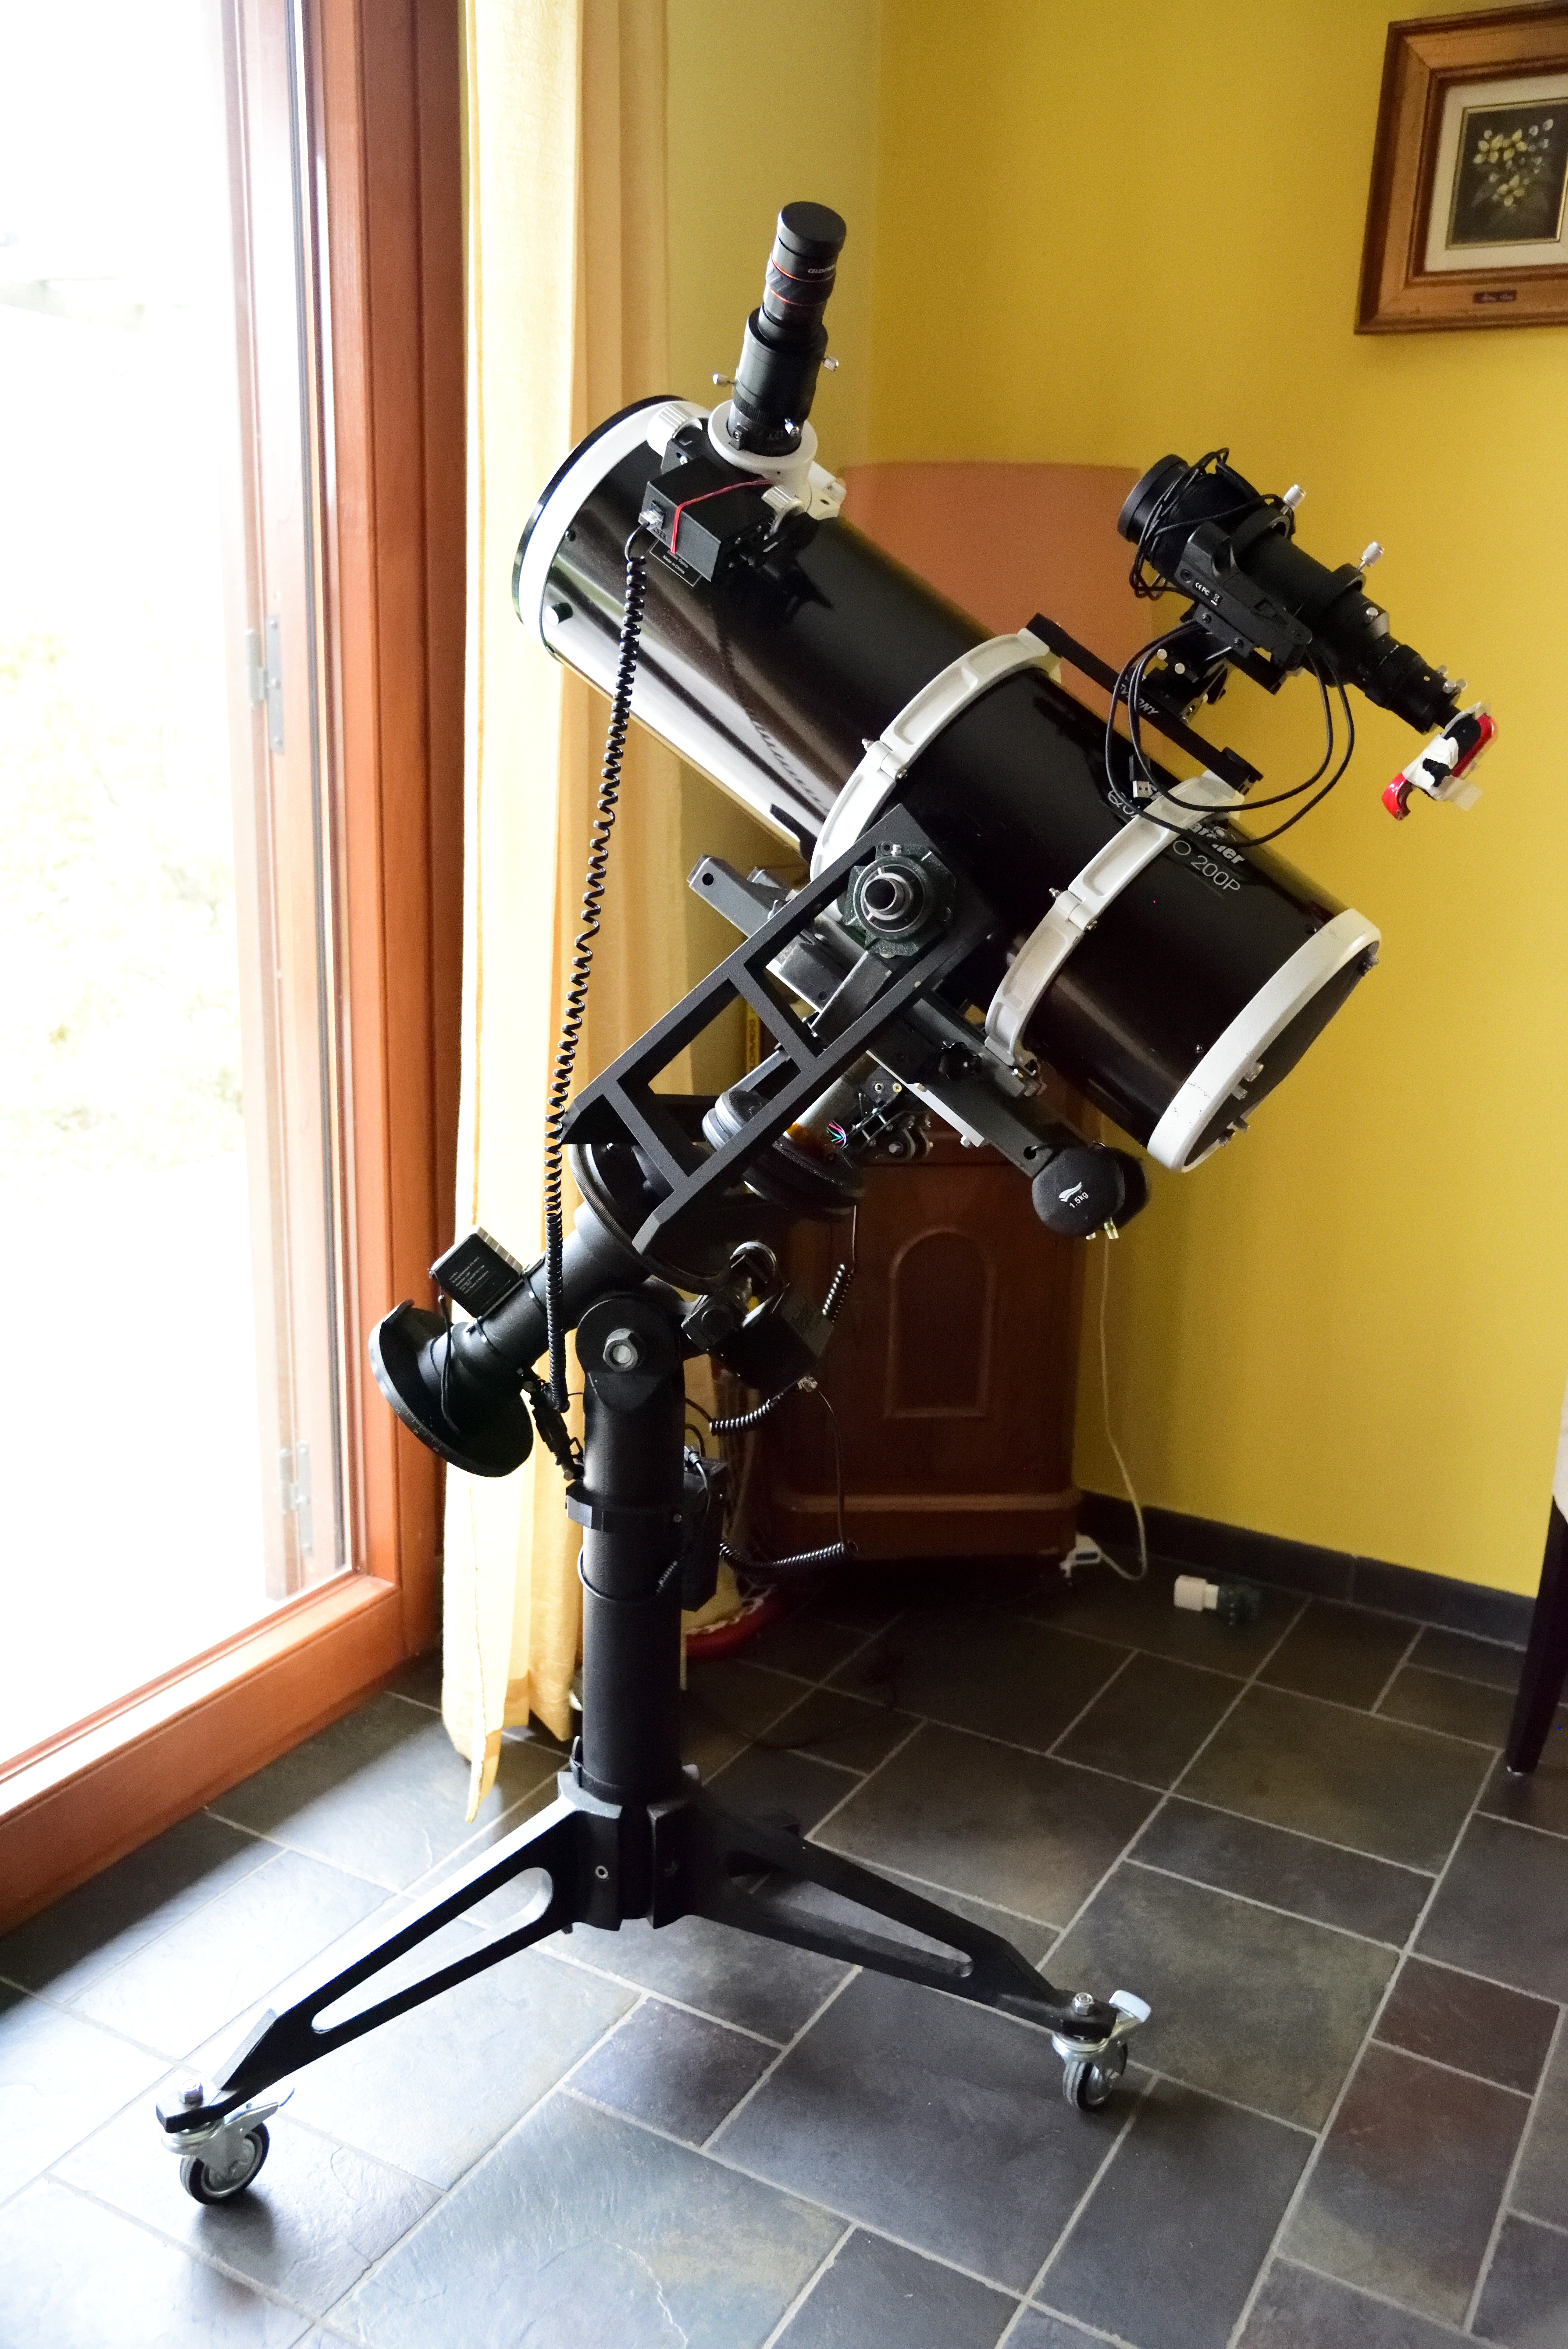
\includegraphics[scale=0.04]{DSC_5264_00001.jpg}
    \captionof{figure}{Final result: our brand-new telescope.}
    \label{fig:final-telescope}
\end{minipage}